% !TEX root= ../main.tex
\externaldocument{discoursegraphs}
\externaldocument{kerneltheory}
\section{Resolving GNF-theories}
\label{sec:Resolving GNF-theories}
In this section, we present an inference system introduced by Walicki in \cite{michal-completeness} which handles clausal theories induced from GNF-theories.

Recall that a theory written in GNF has formulae of the following form:
\begin{align}
  x \lar \bigwedge_{i \in I_x} \neg y_i
\end{align}
Using simple operations only, one can manipulate these formulae into an equivalent set of clauses.
We start by writing the above bi-implication as two implications:
\begin{align}
  x \rightarrow \bigwedge_{i \in I_x} \neg y_i \quad\quad \text{and} \quad\quad x \leftarrow \bigwedge_{i \in I_x} \neg y_i
\end{align}
The first implication can be rewritten in the following way:
\begin{align}
  x \rightarrow \bigwedge_{i \in I_x} \neg y_i
  \quad\Leftrightarrow\quad \neg x \vee \bigwedge_{i \in I_x} \neg y_i
  \quad\Leftrightarrow\quad \bigwedge_{i \in I_x} (\neg x \vee \neg y_i)
  \quad\Leftrightarrow\quad \bigwedge_{i \in I_x} \neg (x \wedge y_i)
\end{align}
The second implication can be rewritten in the following way:
\begin{align}
  x \leftarrow \bigwedge_{i \in I_x} \neg y_i
  \quad\Leftrightarrow\quad x \vee \neg \left( \bigwedge_{i \in I_x} \neg y_i \right)
  \quad\Leftrightarrow\quad x \vee \bigvee_{i \in I_x} y_i
\end{align}
By splitting the conjunction from the first implication up into individual clauses, we get the following two kinds of clauses for every variable $x$ in the GNF theory:
\begin{align}
  \text{OR-clause:}&\quad x \vee \bigvee_{i \in I_x} y_i\\
  \text{NAND-clauses:}&\quad \neg (x \wedge y_i)\text{, for every }i \in I_x
\end{align}
We will treat both the OR-clauses and the NAND-clauses as sets of atoms, denoting NAND-clauses $\neg (x \wedge y)$ as $\overline{xy}$ and OR-clauses $x \vee y_1 \vee y_2 \vee y_3$ as $xy_1y_2y_3$.
This enables us to state things like $\overline{xy} \subset \overline{xyz}$.
A theory will -- as expected -- be a set of OR- and NAND-clauses.

If we interpret the initial GNF-theory as a graph $\mathbf{G}=\langle G,N\rangle$, for every vertex $x \in G$, there will be one OR-clause $\{ x \} \cup N(x)$ and for every edge $\langle x,y \rangle \in N$ there will be a NAND-clause $\overline{xy}$.
The graphs from Example~\ref{ex:3graphs} will have the following clausal theories:
\begin{align}
  \mathcal{T}(\mathbf{G_1}) &= \{ a, \ol{a} \}\\
  \mathcal{T}(\mathbf{G_2}) &= \{ abc, b, c, \ol{ab}, \ol{ac} \}\\
  \mathcal{T}(\mathbf{G_3}) &= \{ abc, bc, \ol{ab}, \ol{bc} \}
\end{align}
Further notation: $A\subseteq G$ denotes an OR-clause while $\ol{A} \subseteq G$ denotes a NAND-clause.
Given a graph $\mathbf{G}=\langle G,N\rangle$, we denote the set of all NAND-clauses induced from the graph as NAND and all induced OR-clauses as OR.
The combined set $\Gamma = NAND + OR$ will be our initial clauses in the inference system.
\subsection{The inference system}
\label{sub:The inference system}
We consider the following inference system, but we will focus mainly on proofs using the Axioms together with the (Rneg) rule.
\begin{align}
  \text{(Ax)} &\quad \Gamma \vdash C, \quad \text{for } C \in \Gamma\\
  \text{(Rneg)} &\quad \frac{ \{ \Gamma \vdash \ol{a_iA_i} \; |\; i \in I \} \quad \Gamma \vdash \{ a_i \; |\; i \in I \} }{ \Gamma \vdash \ol{\bigcup_{i \in I} A_i} }\\
  \text{(Rpos)} &\quad \frac{ \Gamma \vdash A \quad \{\Gamma \vdash B_iK_i \; |\; i \in I \} \quad \{ \Gamma \vdash \ol{a_ik} \; |\; i \in I, k \in K_i \} }{ \Gamma \vdash (A \setminus \{ a_i \; |\; i \in I \} ) \cup \bigcup_{i \in I} B_i }
\end{align}
(Rneg) is creating NAND-clauses from NAND-clauses using OR as a side-condition.
(Rpos) is creating OR-clauses from OR-clauses using NAND as a side-condition.
In (Rneg), $\ol{a_iA_i}$ denotes the NAND $\ol{\{ a_i \} \cup A_i}$ with a potentially empty $A_i$.

The premise of the (Rneg) rule is a set of $I$ NAND-clauses together with one OR-clause with $I$ elements such that each atom $a_i$ in the OR-clause is contained within a NAND-clause, and such that each NAND-clause contains an atom from the OR-clause.
The correspondence between the NAND-clauses and the elements of the OR-clause should in other words be bijective.
The conclusion is the union of all the NAND-clauses without their corresponding atom from the OR-clause.

Here are some examples of incorrect applications of the (Rneg)-rules, followed by some correct applications:
\begin{align}
  (1)\;\;\frac{\ol{ax}\quad\ol{by}\quad\ol{cz}}{\ol{xyz}}abx\quad\quad
  (3)\;\;\frac{\ol{ax}\quad\ol{by}}{\ol{xy}}abx\quad\quad
  (2)\;\;\frac{\ol{ax}\quad\ol{by}\quad\ol{bz}}{\ol{xyz}}abx
\end{align}
(1) is incorrect because the NAND $\ol{cz}$ contains no atoms from the OR $abx$.
(2) is incorrect because the number of NAND-clauses does not match the length of the OR-clause.
(3) is incorrect because there exist no bijective correspondence of the type described above.
\begin{align}
  (4)\;\;\frac{\ol{ax}\quad\ol{by}\quad\ol{cz}}{\ol{xyz}}abc\quad\quad
  (5)\;\;\frac{\ol{ax}\quad\ol{b}}{\ol{x}}ab\quad\quad
  (6)\;\;\frac{\ol{ax}\quad\ol{by}\quad\ol{xyz}}{\ol{xyz}}abx
\end{align}
The three above applications are all correct, since all the atoms in each OR-clause get matched to exactly one NAND-clause in such a way that no NAND-clause stays unmatched.

We set no restrictions on the number and cardinality of our clauses, meaning that there might be an infinite number of clauses, and both the OR-clauses and the NAND-clauses might be either finite or infinite in size.
Note that an infinite graph gives infinitely many NAND-clauses, while an infinitary graph also gives us infinitely long OR-clauses.

We study the refutation system that arises from the Axioms and the (Rneg)-rule, calling it Neg.
It is shown in \cite{michal-completeness} that Neg is sound and refutationally complete for theories with only a countable number of OR-clauses.
Soundness gives us that proving $\ol{C}$ for any $C \subseteq G$ implies that the vertices in $C$ cannot all be assigned 1 in the graph model.
Refutational completeness gives us that whenever a graph/theory is inconsistent, we are able to prove $\varnothing$ in Neg.

Note that Neg is not generally complete.
The following inconsistent graph exemplifies this:\par
\begin{figure}[!h]
  \centering
  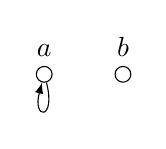
\begin{tikzpicture}
    [
    point/.style={circle,draw,inner sep=0pt,minimum size=2mm}
    ]
    \node (1) at (0,0) [point, label=above:$a$] {};
    \node (2) at (1,0) [point, label=above:$b$] {};
    \draw [-latex, loop below] (1) to (1);
  \end{tikzpicture}
  \caption{}
  \label{fig:neg_not_complete}
\end{figure}
Bacause of the loop on vertex $a$, the graph has no solutions.
We therefore have $\vDash \ol{b}$, but we are unable to prove $\ol{b}$ in Neg.
\subsection{Inconsistency of the Yablo-graph}
\label{sub:Inconsistency of the Yablo-graph}
The inconsistency of the Yablo-graph is easily proven using Neg only.
Since every vertex $x_i$ (using the notation from Figure~\ref{fig:yablo-graph}) has an edge to each vertex $x_j$ where $j > i$, we get that every pair of distinct vertices is connected by an edge.
This means that our set of axioms from the Yablo-graph looks like this:
\begin{align}
  \text{NAND} = \{ \ol{x_ix_j} \; |\; i < j\}
  \quad\quad\quad
  \text{OR} = \{ x_ix_{i+1}x_{i+2}\dots \; |\; i \in \mathbb{N}\}
\end{align}
For any vertex $x_i$ from the Yablo-graph, we are now able to prove $\ol{x_i}$ in the following way:
\begin{prooftree*}
  \Hypo{\ol{x_ix_{i+1}}}
  \Hypo{\ol{x_ix_{i+2}}}
  \Hypo{\ol{x_ix_{i+3}}}
  \Hypo{\dots}
  \Infer4[$x_ix_{i+1}x_{i+2}\dots$]{\ol{x_i}}
\end{prooftree*}
Proving $\varnothing$ is now simple:
\begin{prooftree*}
  \Hypo{\dots}
  \Infer1{\ol{x_1}}
  \Hypo{\dots}
  \Infer1{\ol{x_2}}
  \Hypo{\dots}
  \Infer1{\ol{x_3}}
  \Hypo{\dots}
  \Infer4[$x_1x_2x_3\dots$]{\varnothing}
\end{prooftree*}
A less trivial inconsistency proof is the one of the \textit{Stretched Yablo-graph}.
This proof can be found in Appendix~\ref{sec:Inconsistency of Stretched Yablo} together with the definition of Stretched Yablo.

It is worth mentioning that even though our focus has been -- and will be -- on theories originating from graphs, the results on soundness and completeness holds for any theory consisting of a set of NANDs and a set of ORs.

An example of this is the pigeonhole problem which easily can be represented as a set of NAND- and OR-clauses, but does not directly correspond to a graph (it can of course be translated to a graph theory, like any other propositional theory).
A Neg-proof of the pigeonhole principle can be found in Section~\ref{sub:Proving the pigeonhole principle}.
